\documentclass{article}
\usepackage{tikz}
\usepackage{amsmath}
\usetikzlibrary{angles,quotes}
\usetikzlibrary{decorations.pathmorphing,calc}
\begin{document}
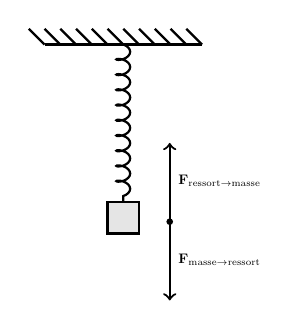
\begin{tikzpicture}[scale=1]
% Paramètres
\def\ressortL{2}   % longueur du ressort
\def\masseH{0.4}   % hauteur de la masse
\def\masseL{0.4}     % largeur de la masse
\def\x{0}
\def\dx{0.5}
\def\w{0.3}
\def\h{0.5}
\def\F{1}
\def\y{-2}
\def\dy{0}
% Support (plafond)
\draw[thick] (-1,0) -- (1,0);
\foreach \x in {-1,-0.8,...,1} {
  \draw[thick] (\x,0) -- (\x-0.2,0.2);
}
% Ressort vertical
\draw[
  thick,
  decorate,
  decoration={coil, segment length=5.5pt, amplitude=2.5pt}
] (0,0) -- (0,-\ressortL);
% Masse verticale
\draw[thick, fill=gray!20]
(-\masseL/2,-\ressortL-\masseH)
rectangle
(\masseL/2,-\ressortL);
% Point d’application de la force
\coordinate (P) at (\x+\dx+0.3*\w,\y+\dy-0.5*\h);
% Force arrow
\draw[thick, ->] (\x+\dx+0.3*\w,\y+\dy-0.5*\h)
 -- ++(0,\F)
 node[midway,right=18,above=-3.5,scale=0.5]
 {$\mathbf{F_{\text{ressort}\rightarrow\text{masse}}}$};
\draw[thick, ->] (\x+\dx+0.3*\w,\y+\dy-0.5*\h)
 -- ++(0,-\F)
 node[midway,right=18,above=-3.5,scale=0.5]
 {$\mathbf{F_{\text{masse}\rightarrow\text{ressort}}}$};
% Point matérialisant le point d’application
\fill (P) circle (1.2pt);
\end{tikzpicture}

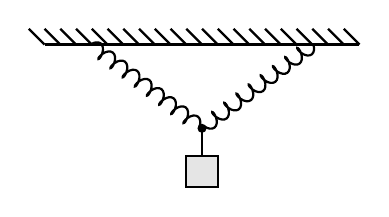
\begin{tikzpicture}[scale=1]
%========================
% Paramètres
%========================
\def\ressortL{2}   % longueur du ressort
\def\masseH{0.4}   % hauteur de la masse
\def\masseL{0.4}     % largeur de la masse
\def\angle{45}     % demi-angle (90° au total)
% ============ AJOUT ============
\def\barreV{0.35}  % longueur de la barre verticale
\def\rayonPt{0.05} % rayon du point (rotule)
% ===============================
% Plafond
%========================
\draw[thick] (-2,0) -- (2,0);
\foreach \x in {-2,-1.8,...,2} {
  \draw[thick] (\x,0) -- (\x-0.2,0.2);
}
%========================
% Points géométriques
%========================
\coordinate (A) at ({-\ressortL*sin(\angle)}, 0);
\coordinate (B) at ({\ressortL*sin(\angle)}, 0);
\coordinate (C) at (0, {-\ressortL*cos(\angle)});
% ============ AJOUT ============
% Point commun d’arrivée des deux ressorts
\coordinate (C) at (0, {-\ressortL*cos(\angle)+\barreV});
% Point d’attache masse / barre
\coordinate (D) at (0, {-\ressortL*cos(\angle)});
% ===============================
% ============ AJOUT ============
% Point commun ressorts / barre
\coordinate (C) at (0, {-\ressortL*cos(\angle)+\barreV});
% Point d’attache barre / masse
\coordinate (D) at (0, {-\ressortL*cos(\angle)});
%========================
% Ressorts obliques
%========================
\draw[
  thick,
  decorate,
  decoration={coil, segment length=5.5pt, amplitude=2.5pt}
] (A) -- (C);
\draw[
  thick,
  decorate,
  decoration={coil, segment length=5.5pt, amplitude=2.5pt}
] (B) -- (C);
% Barre verticale
%========================
% ============ AJOUT ============
\draw[thick] (C) -- (D);
% ===============================
% Point (rotule) au point commun
\filldraw[black] (C) circle (\rayonPt);
% Masse suspendue
%========================
\draw[thick, fill=gray!20]
(-\masseL/2, {-\ressortL*cos(\angle)-\masseH})
rectangle
(\masseL/2, {-\ressortL*cos(\angle)});
\end{tikzpicture}


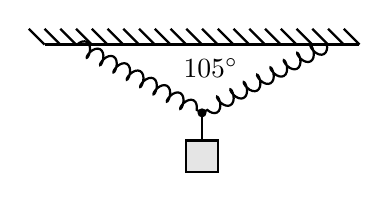
\begin{tikzpicture}[scale=1]

%========================
% Paramètres
%========================
\def\ressortL{2}    % longueur du ressort
\def\masseH{0.4}    % hauteur de la masse
\def\masseL{0.4}    % largeur de la masse
\def\angle{52.5}    % demi-angle -> 105° d’ouverture totale
\def\barreV{0.35}   % longueur de la barre verticale
\def\rayonPt{0.05}  % rayon du point (rotule)

%========================
% Plafond
%========================
\draw[thick] (-2,0) -- (2,0);
\foreach \x in {-2,-1.8,...,2} {
  \draw[thick] (\x,0) -- (\x-0.2,0.2);
}

%========================
% Points géométriques
%========================
\coordinate (A) at ({-\ressortL*sin(\angle)}, 0);
\coordinate (B) at ({\ressortL*sin(\angle)}, 0);

% Point commun ressorts / barre
\coordinate (C) at (0, {-\ressortL*cos(\angle)+\barreV});

% Point d’attache barre / masse
\coordinate (D) at (0, {-\ressortL*cos(\angle)});
%========================
% Ressorts obliques
%========================
\draw[
  thick,
  decorate,
  decoration={coil, segment length=5.5pt, amplitude=2.5pt}
] (A) -- (C);
\draw[
  thick,
  decorate,
  decoration={coil, segment length=5.5pt, amplitude=2.5pt}
] (B) -- (C);

%========================
% Barre verticale
%========================
\draw[thick] (C) -- (D);
%========================
% Point (rotule)
%========================
\node at (0.11,-0.30) {$105^\circ$};
\filldraw[black] (C) circle (\rayonPt);

%========================
% Masse suspendue
%========================
\draw[thick, fill=gray!20]
(-\masseL/2, {-\ressortL*cos(\angle)-\masseH})
rectangle
(\masseL/2, {-\ressortL*cos(\angle)});

\end{tikzpicture}



\end{document}